\chapter{Motivation}\label{chap:motivation_wf}

To create a workflow enclosing multiple paths where each path comprises of multiple tools is a complex task. The users need to keep knowledge of the tools that can come next. These next tools should be compatible to the previous one which is a necessary criterion for the tools to be connected on the canvas of Galaxy workflow editor. No two incompatible tools can connect to each other. This knowledge of compatibility is a must which can be gained only through experience. A user who is new to the Galaxy platform and is not aware of the existing tools, to create a workflow can be a labourious and time-consuming effort. 

\begin{figure}[h]
\begin{centering}
    {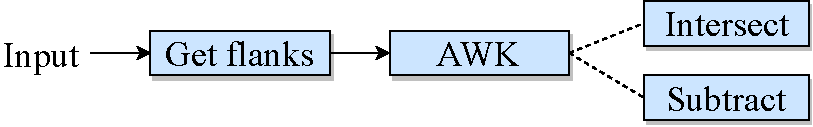
\includegraphics[scale=0.7]{figures/multiple_next_tools_45cee2961bc05b20.pdf}}
    \caption[Multiple next tools]{\textbf{Mulitple next tools}: The image shows a part of a workflow where one tool can connect to more than one tool.}
\end{centering}
\end{figure}

In figure 34, we can see that a tool "AWK" can connect to two tools, "Intersect" and "Subtract". The number of next tools can vary from tool to tool. Some tools can have just one next tool but others can have many different next tools they can connect to. To impart the knowledge of the next tools (for a tool or a sequence of tools) at each stage of creating a workflow, we propose to build a prediction system. It would recommend a set of next possible tools to a user whenever he/she chooses and connects a tool to a workflow. It would scale down the size of the collection of next tools to choose from and thereby we expect a reduction in the time taken to create workflows. Many users create and store their workflows on Freiburg Galaxy server. We intend to learn the tools connecting patterns present in these workflows as long sequences of tools using machine learning and predict next tools.